\section{Design}

\subsection{146. LRU Cache}

\paragraph{\color{white} \colorbox{Mahogany}{Description}}
Design and implement a data structure for Least Recently Used (LRU) cache. It should support the following operations: get and put.
\begin{itemize}
    \item get(key) - Get the value (will always be positive) of the key if the key exists in the cache, otherwise return -1.
    \item put(key, value) - Set or insert the value if the key is not already present. When the cache reached its capacity, it should invalidate the least recently used item before inserting a new item.
\end{itemize}

Follow up:
Could you do both operations in O(1) time complexity?

\paragraph{\color{white} \colorbox{OliveGreen}{Solution}}
\underline{Code Hints:}
\begin{itemize}
    \item A linked list (use \mintinline{cpp}|ListNode| provided by LeetCode or \mintinline{cpp}|std::list<int>::iterator|) to store keys in LRU order.
    \item A map to find values and their positions in the linked list by keys.
\end{itemize}
\begin{figure}[ht]
    \centering
    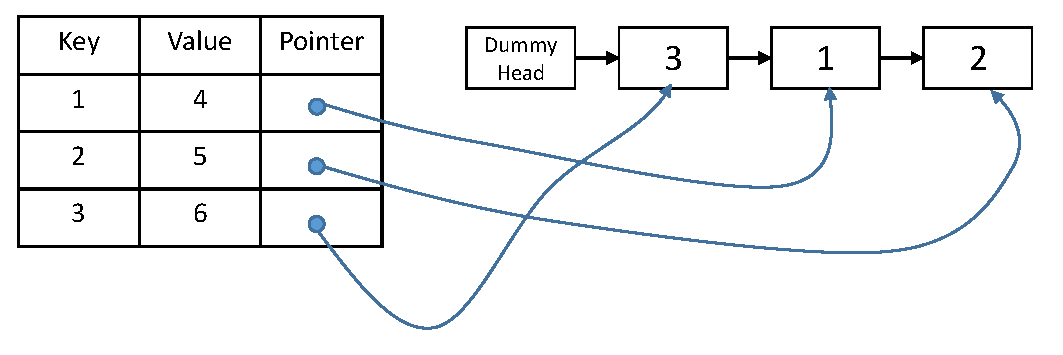
\includegraphics[width=13cm]{lru_cache}
    \label{fig:lru_cache}
\end{figure}